%! TeX program = xelatex
%! TEX-TS program = xelatex
\documentclass[aspectratio=169,xcolor={dvipsnames}]{beamer}

\input{/home/shiroha/Documents/latex/templates/slides/metro_lm.tex}

% % references
% \setbeamertemplate{bibliography item}[text] % change reference icon to number
% \setbeamertemplate{frametitle continuation}{} % remove 'i' before frametitle 'Reference'
% \usepackage[backend=biber,style=chem-acs]{biblatex}
% \usepackage{bibentry} % enable direct bibentry print
% \addbibresource{references.bib}


% title page
\newcommand\mail{has015@ucsd.edu}
\title{CHEM 6B WI24 F02-F06}
\subtitle{Week 3: work and heat}
\author{TA: Haoran Sun (\href{mailto:\mail}{\mail})}
\institute{University of California, San Diego}
\date{January 19, 2024}

\begin{document}

\maketitle

% \begin{frame}{Outline}
%     \tableofcontents
% \end{frame}

\begin{frame}[t]
    \frametitle{State function}
    \begin{itemize}
        \item Definition: a property whose value doesn't depend on the path taken 
            to reach that specific value.
            \begin{itemize}
                \item Examples: energy $E$, volume $V$, temperature $T$, pressure $P$,
                    number of particles $n$, {\color{gray} entropy $S$}
                \item Counterexamples: work $W$, heat $Q$
            \end{itemize}

        \item<2> Intuitively, imagine the following scenario: during weekdays, 
            you will come to campus to take courses.
            \begin{itemize}
                \item You can commute between two locations by car, bike, walk,
                    and by different path. 
                \item \textbf{Location} is a state function, independent from path you take.\\
                    9500 Gilman Dr, La Jolla, CA 92093.
                \item \textbf{Way \& path to commute} is not a state function.
            \end{itemize}
    \end{itemize}
\end{frame}

\begin{frame}[t]
    \frametitle{Energy change of a system}
    \begin{itemize}
        \item Energy change of a system equals to 
            the work done on the system $\Delta W$ and heat $\Delta Q$ absorb
            by the system.
            \begin{align}
                \Delta E &= \Delta W + \Delta Q
            \end{align}
        \item For an ideal gas system, one has $\Delta W = -P\d V$
            and $\Delta Q = C\d T$, where $C$ is the heat capacity {\color{gray}
            at constant volume.}
            \begin{align}
                \Delta E &= \underbrace{-P\Delta V}_{\mathclap{\Delta W}} + 
                    \underbrace{C\Delta T}_{\mathclap{\Delta Q}}
            \end{align}
    \end{itemize}
\end{frame}

\begin{frame}[t]
    \frametitle{Sign of energy/work/heat change}
    \begin{itemize}
        \item If $\Delta E$/$\Delta W$/$\Delta Q > 0$, the system \ul{gain}
            energy/work/heat from the outside.
        \item If $\Delta E$/$\Delta W$/$\Delta Q < 0$, the system \ul{lose}
            energy/work/heat to the outside.
        \item Recall $\Delta W = -P\Delta V$
    \end{itemize}
    Week 3, problem 4
    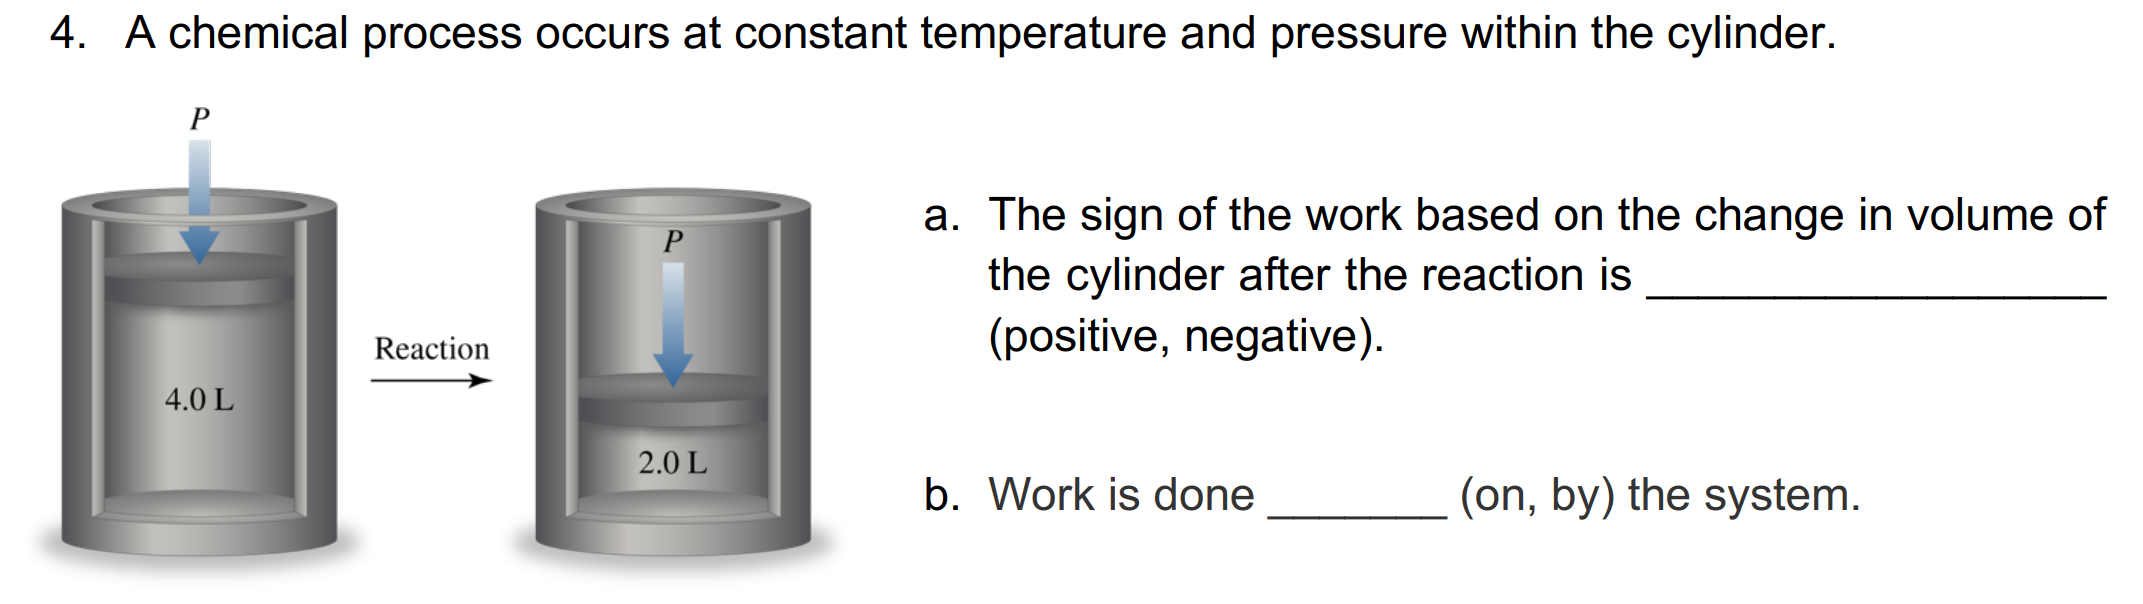
\includegraphics[width=\textwidth]{q4.png}
\end{frame}


\begin{frame}[t]
    \frametitle{Temperature change caused by heat transfer}
    \only<1>{
    Heat capacity
    \begin{itemize}
        \item Recall $\Delta Q = C\Delta T\Rightarrow \Delta T = \frac{\Delta Q}{C}$.
        \item Exercise: let the heat capacity of a $\SI{10}{\gram}$ substance 
            be $C = \SI{10}{\joule\cdot\kelvin^{-1}}$.
            \begin{itemize}
                \item How would the temperature change if this substance gain $\SI{100}{\joule}$ heat?
                \item How would the temperature change if this substance lose $\SI{100}{\joule}$ heat?
            \end{itemize}
    \end{itemize}}
    \only<2>{Specific heat capacity
    \begin{itemize}
        \item Now define specific heat capacity by $c = C/m\Leftrightarrow
            C = mc$, where $m$ is the mass of the substance.
            The physical meaning is the heat absorbed per unit mass.
        \item From $\Delta Q = C\Delta T$ one can then derive
            \begin{align}
                \Delta Q &= C\Delta T\Rightarrow
                \Delta Q = mc\Delta T
                \Rightarrow \Delta T = \frac{Q}{mc}
            \end{align}
        \item Exercise: let the specific heat capacitiy of a substance be 
            $c = \SI{5}{J\cdot\gram^{-1}\cdot\kelvin^{-1}}$
            \begin{itemize}
                \item How would the temperature change if 10 gram of such 
                    substance absorbs $\SI{1000}{\joule}$ heat?
            \end{itemize}
    \end{itemize}}

\end{frame}

\begin{frame}[t]
    Week 3, problem 5
    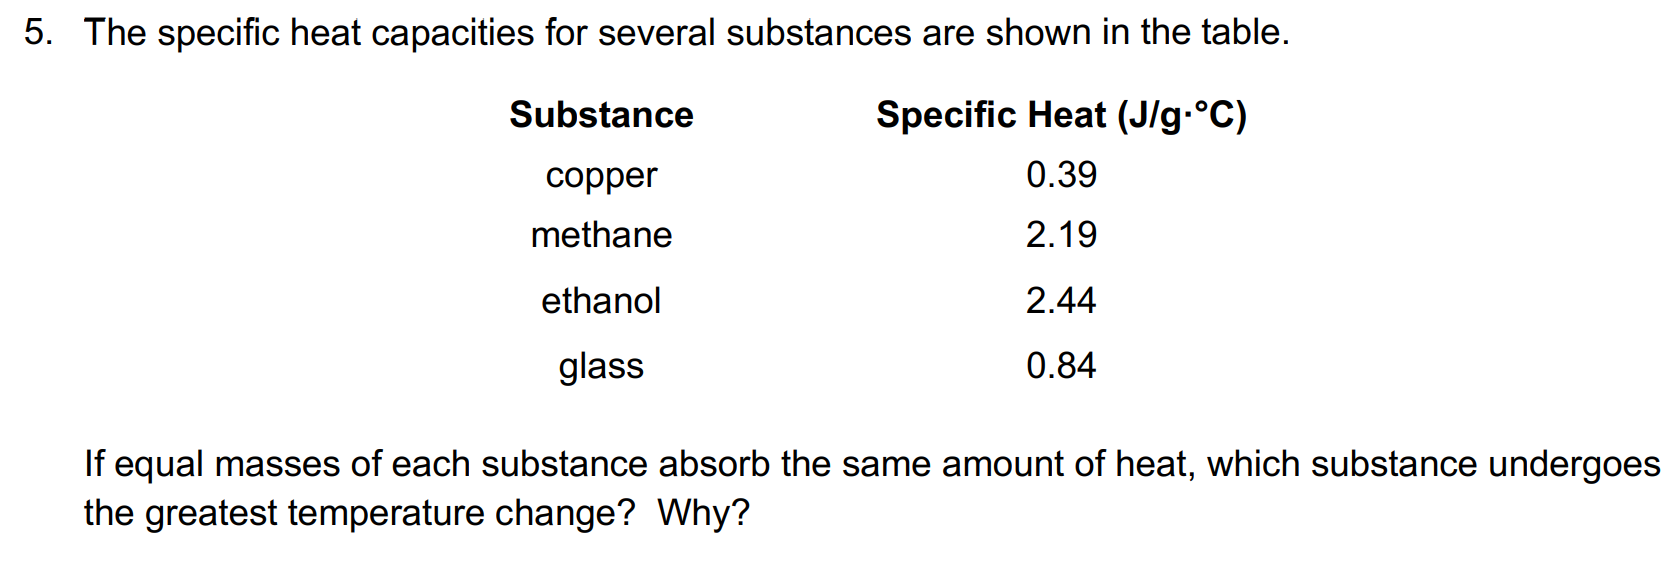
\includegraphics[width=0.8\textwidth]{q5.png}
\end{frame}

\begin{frame}[t]
    Week 3, problem 6
    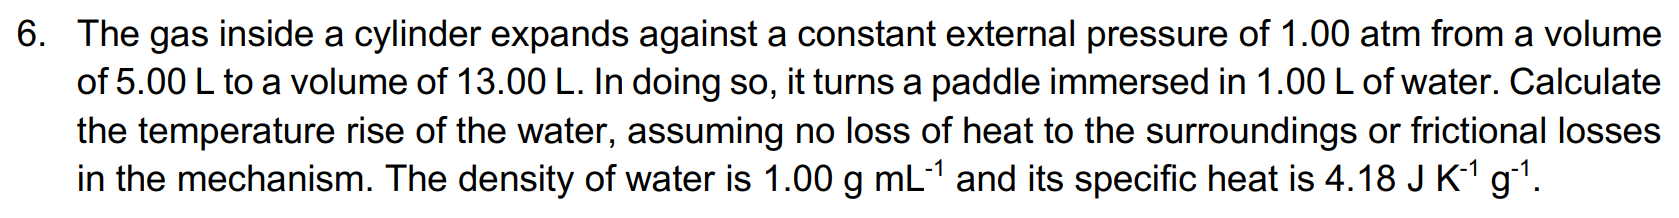
\includegraphics[width=\textwidth]{q6.png}
\end{frame}

% % reference page
% \begin{frame}[allowframebreaks]
%     \frametitle{References}
%     \nocite{*}
%     \printbibliography
% \end{frame}

\end{document}



